\documentclass[tikz]{standalone}


\usepackage{tikz}
\usetikzlibrary{calc}
\usepackage{amsmath}


\definecolor{lensblue}{HTML}{95D1FF}


\begin{document}

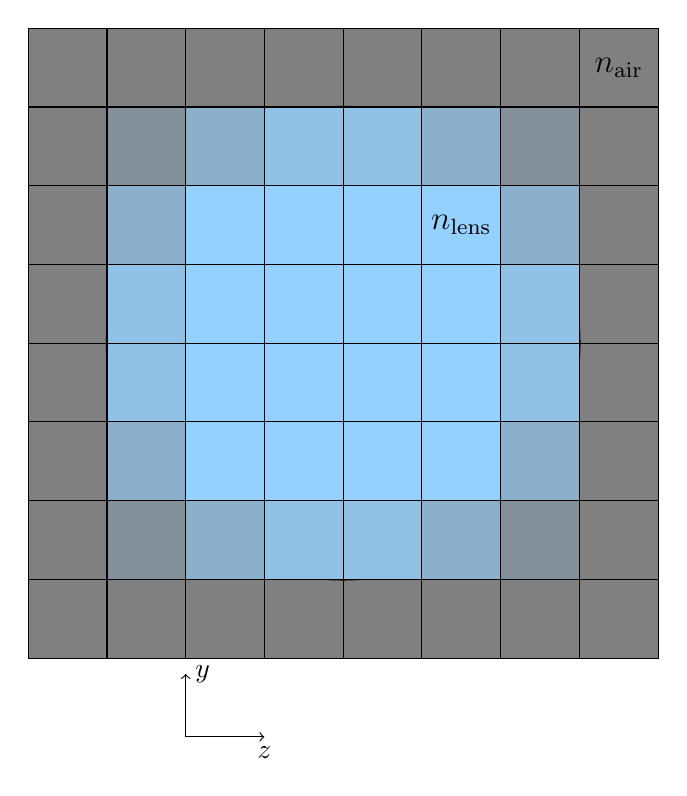
\begin{tikzpicture}
  \draw[fill=gray] (-4, -4) rectangle (4, 4);
  \draw[thick, fill=lensblue] (0,0)  circle (3);
  \node at (3.5,3.5) {\large $n_\text{air}$};
  \node at (1.5,1.5) {\large $n_\text{lens}$};


  \fill[color=lensblue!20!gray] (-3, -3) rectangle (-2, -2);
  \fill[color=lensblue!20!gray] (3, 3) rectangle (2, 2);
  \fill[color=lensblue!20!gray] (3, -3) rectangle (2, -2);
  \fill[color=lensblue!20!gray] (-3, 3) rectangle (-2, 2);


  \fill[color=lensblue!60!gray] (-2, -3) rectangle (-1, -2);
  \fill[color=lensblue!60!gray] (-3, -2) rectangle (-2, -1);
  \fill[color=lensblue!60!gray] (2, 3) rectangle (1, 2);
  \fill[color=lensblue!60!gray] (3, 2) rectangle (2, 1);
  \fill[color=lensblue!60!gray] (2, -3) rectangle (1, -2);
  \fill[color=lensblue!60!gray] (3, -2) rectangle (2, -1);
  \fill[color=lensblue!60!gray] (-2, 3) rectangle (-1, 2);
  \fill[color=lensblue!60!gray] (-3, 2) rectangle (-2, 1);


  \fill[color=lensblue!80!gray] (-1, -3) rectangle (0, -2);
  \fill[color=lensblue!80!gray] (1, -3) rectangle (0, -2);
  \fill[color=lensblue!80!gray] (-1, 3) rectangle (0, 2);
  \fill[color=lensblue!80!gray] (1, 3) rectangle (0, 2);

  \fill[color=lensblue!80!gray] (-3, -1) rectangle (-2, 0);
  \fill[color=lensblue!80!gray] (-3, 1) rectangle (-2, 0);
  \fill[color=lensblue!80!gray] (3, -1) rectangle (2, 0);
  \fill[color=lensblue!80!gray] (3, 1) rectangle (2, 0);



  \foreach \i in {-4, -3, -2, -1, 0, 1, 2, 3, 4}
  {
    \draw[-] (-4, \i) -- (4, \i);
    \draw[-] (\i, -4) -- (\i, 4);
  }  

  \draw[->] (-2, -5) -- (-1, -5) node [right, below] {$z$};
  \draw[-> ](-2, -5) -- (-2, -4.2) node [right, right] {$y$};

\end{tikzpicture}
\end{document}
